\input{configuration}

\title{Lecture 19 --- Real-Time Scheduling Algorithms }

\author{Jeff Zarnett \\ \small \texttt{jzarnett@uwaterloo.ca}}
\institute{Department of Electrical and Computer Engineering \\
  University of Waterloo}
\date{\today}


\begin{document}

\begin{frame}
  \titlepage

 \end{frame}


\begin{frame}
\frametitle{Onward Then}

We talked about what makes scheduling for real-time systems different.

We already covered timeline scheduling.

Let's go back to the uniprocessor world to start...

\end{frame}


\begin{frame}
\frametitle{Earliest Deadline First}

The earliest deadline first algorithm is, presumably, very familiar to students. 

\begin{center}
	\includegraphics[width=0.5\textwidth]{images/deadlines.jpg}
\end{center}

\end{frame}


\begin{frame}
\frametitle{Earliest Deadline First}

Assignment due today, an assignment due next Tuesday, and an exam next month, then you may choose to schedule these things by their deadlines. 

Do the assignment due today first. 

After completing an assignment, decide what to do next (probably the new assignment, but perhaps a new task has arrived in the meantime?) and start.


\end{frame}

\begin{frame}
\frametitle{Earliest Deadline First}

The principle is the same for the computer. 

Choose the task with the soonest deadline; if there is a tie, then random selection between the two will be sufficient (or other criteria may be used). 

\end{frame}

\begin{frame}
\frametitle{Earliest Deadline First}

If there exists some way to schedule all the tasks such that all deadlines are met, this algorithm will find it. 

If a task is executing and another task arrives with a sooner deadline, the currently executing task should be suspended and the new task scheduled. 

This may mean a periodic task being preempted by an aperiodic/sporadic task.

\end{frame}

\begin{frame}
\frametitle{Implementing EDF}

A priority queue is reasonable...

Sort by deadline? Does that account for task type?

Ah, but what if we're overloaded...?

\end{frame}

\begin{frame}
\frametitle{Deadline Interchange}

This deadline-based approach is subject to a problem that very much resembles priority inversion.

\begin{center}
	\includegraphics[width=0.4\textwidth]{images/takeit.jpg}
\end{center}

\end{frame}

\begin{frame}
\frametitle{Deadline Interchange}
Suppose a task $A$ holds a resource and then a new task $B$ arrives that also needs that resource, but has a sooner deadline than $A$. 

If there are other tasks $C, D, E$... that also want this resource, $A$ could be waiting a long time to proceed.

Even if $B$ misses its deadline!

\end{frame}

\begin{frame}
\frametitle{Deadline Interchange}

The best way to make that happen would be to assign to $A$ a new deadline, specifically the soonest deadline from all the tasks waiting for it. 

Doesn't that look like priority inheritance?

\end{frame}


\begin{frame}
\frametitle{Least Slack First}

A similar algorithm to earliest deadline first, is least slack first.

\begin{center}
	\includegraphics[width=\textwidth]{images/slack.png}
\end{center}


\end{frame}

\begin{frame}
\frametitle{Least Slack First}

\alert{Slack}: how long a task can wait before it must be scheduled to meet a deadline.

If a task will take 10~ms to execute and its deadline is 50~ms away, then there are (50 - 10) = 40~ms of slack time remaining.

Start the task before 40~ms are expired if we want to be sure that it will finish. 

\end{frame}

\begin{frame}
\frametitle{Least Slack First}
This does not mean, however, that we necessarily want to wait 40~ms before starting the task (even though many students tend to operate on this basis). 

All things being equal, we prefer tasks to start and finish as soon as possible. 

It does, however, give us an indication of what tasks are in most danger of missing their deadlines and should therefore have priority.

\end{frame}

\begin{frame}
\frametitle{Rate-Monotonic Scheduling}

The name doesn't explain this one super well.

EDF and LSF don't really consider priorities.

Rate-Monotonic scheduling is based around the idea of basing priority on the period -- tasks that execute more often are given higher priority.

\end{frame}

\begin{frame}
\frametitle{Not Quite Optimal}

This algorithm is, however, not perfect.

It's possible to fail to schedule things in such a way that all tasks meet their deadlines even if utilization is less than 1.

Example: $n$ periodic tasks with the form $(C_{k}, \tau _{k})$: (1, 4), (3, 7), and (3, 10).

\end{frame}

\begin{frame}
\frametitle{That's Not Supposed to Happen}


Utilization is less than 1 so it should be possible to solve this one: ($1/4 + 3/7 + 3/10 = 137/140$). 

Earliest Deadline First would have been able to schedule this such that it met all deadlines. 

\begin{center}
	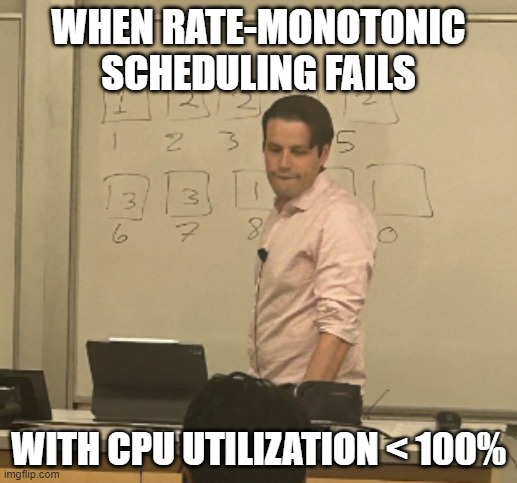
\includegraphics[width=0.4\textwidth]{images/rate-monotonic.jpg}
\end{center}

\end{frame}

\begin{frame}
\frametitle{Take the Test}

To figure out if it's possible to schedule things, there's a test. 

It turns out that it's very difficult to do this dynamically in real-time, so we have to use a less-precise formula.

\begin{center}
	$\Pi^{n}_{k=1}( 1 + \dfrac{c_k}{\tau _k}) \leq 2$.
\end{center}

Remember: uncertain success is not certain failure.

\end{frame}

\begin{frame}
\frametitle{Deadline Monotonic}

A variant of this is deadline-monotonic scheduling, in which case priority is assigned based on deadlines.

The task with the shortest deadline is assigned the highest priority.

\end{frame}

\begin{frame}
\frametitle{Aperiodic Servers}

\begin{center}
	\includegraphics[width=0.3\textwidth]{images/witchking.jpg}
\end{center}

A task with a soft deadline is challenging to schedule here, because it's hard for the scheduler to know whether a task is soft- or hard-real time.

One possibility is to say that aperiodic or soft-deadline tasks are always lower in priority than any firm- or hard-real time task.

\end{frame}

\begin{frame}
\frametitle{Polling Server}

A polling server is, in its own way, a little container in which aperiodic tasks occur.

\begin{center}
	\includegraphics[width=0.3\textwidth]{images/redhour.jpg}
\end{center}

The server is itself a hard-deadline periodic task with a fixed execution time budget and a deadline equal to its period.

\end{frame}

\begin{frame}
\frametitle{Periodic Server}

\begin{center}
	\includegraphics[width=0.4\textwidth]{images/periodic-server.jpg}
\end{center}

During the execution time of the server task, the aperiodic tasks waiting will run sequentially.

\end{frame}

\begin{frame}
\frametitle{Too Much or Too Little}

If there are too many tasks or they otherwise take too long and they do not finish, the aperiodic tasks just carry over to the next time the server runs. 

If there are not enough aperiodic tasks and there's time left over, just end the server task execution (throw away the extra time) and let something else run.

\end{frame}

\begin{frame}
\frametitle{Periodic Server Analogy}

\begin{center}
	\includegraphics[width=0.75\textwidth]{images/lunchtime.jpg}
\end{center}

Do you have to use your lunch break for eating lunch?

\end{frame}

\begin{frame}
\frametitle{Multiple Servers}

We can have different servers that work on different kinds of tasks.

In the lunch break analogy, what if there's lunch breaks and coffee breaks?

\hfill \includegraphics[width=0.3\textwidth]{images/duo-peeking.png}


\end{frame}

\begin{frame}
\frametitle{Does It Work?}
Polling server does not affect the ability of the system to complete the hard-deadline tasks.

The background server's behaviour is predictable!

Downside: response time for aperiodic tasks.

\end{frame}

\begin{frame}
\frametitle{Variant: Deadline-Deferrable}

Improved version: deferrable server.

Instead of throwing away the time budget if it's unused at the end of the period and there's nothing to do, save that leftover time.

Either the time is used up or eventually expires.

\end{frame}

\begin{frame}
\frametitle{Deferrable Server}
Finished with 40\% budget remaining?

Polling server: Throw it away.\\
\quad... Back to work even if lunch finished in 45 minutes; 15 mins lost.

Deferrable server: Keep it until the end of the period.\\
\quad Save those 15 minutes for later in the day, but can't carry over to tomorrow.

\end{frame}

\begin{frame}
\frametitle{Reminder: Consult a Lawyer}

\begin{center}
	\includegraphics[width=0.5\textwidth]{images/attorneys.jpg}
\end{center}

Note that none of this is a substitute for legal advice from an employment lawyer about the rules \& regulations around legally required breaks during the workday.

\end{frame}

\begin{frame}
\frametitle{Variant 2: Deadline-Sporadic}

Next idea: sporadic server!


Instead of losing the extra unused period, it can be saved, indefinitely. 

The replenishment of the budget forces execution to be spread out more evenly.

\end{frame}

\begin{frame}
\frametitle{Why Does Spreading It Matter?}

\begin{center}
	\includegraphics[width=0.4\textwidth]{images/balanced.jpg}
\end{center}

\begin{center}
	\includegraphics[width=0.7\textwidth]{images/ttc.png}
\end{center}

\end{frame}

\begin{frame}
\frametitle{Spreading It Out}

Execution time for the server is broken down into chunks.

When a chunk is depleted, it's scheduled for replenishment in the future.

\end{frame}

\begin{frame}
\frametitle{Replenishment is Familiar Maybe}

\begin{center}
	\includegraphics[width=0.4\textwidth]{images/duolingo-hearts.png}
	\includegraphics[width=0.4\textwidth]{images/aws.jpg}
\end{center}

\end{frame}

\begin{frame}
\frametitle{Variant 3: Deadline Exchange Server}
Like Deadline-Deferrable server, but simplifies tracking the chunks.

Any remaining execution time is discarded when the request queue is empty and the wait for replenishment is based on the last chunk of execution time used.

This is simpler to implement since there's only ever one replenishment to track and the replenishment is always the full quota. 

\end{frame}

\begin{frame}
\frametitle{But Does it Work?}

Simulation studies show that different forms of the period server approach are effective for different workloads.

Remember: it's possible to have different servers configured for different aperiodic tasks to give the best balance of prioritization and performance.

\end{frame}

\begin{frame}
\frametitle{Multiprocessor Math}

Now it's time to get out of uniprocessor and into multiprocessor scheduling.

Task $\rightarrow$ things that need doing.

Job $\rightarrow$ specific instance of the task to run.

\end{frame}

\begin{frame}
\frametitle{Three Relevant Questions}

Is preemption permitted?

Is job migration permitted?

Is job parallelism permitted?

\end{frame}

\begin{frame}
\frametitle{This Is Mine And You Can't Have It}

Dedicated CPUs are an option, possibly with manual assignment. 

That makes it more like the uniprocessor situation.

\begin{center}
	\includegraphics[width=0.4\textwidth]{images/yearsofexperience.jpg}
\end{center}

\end{frame}

\begin{frame}
\frametitle{Computer, Please Help}
Asking the computer to do it? This is one of those NP-Complete problems.

Doing so in advance for an all-periodic system is doable.

For systems with sporadic and aperiodic tasks, the cost of doing this math might be prohibitive at runtime. 

\end{frame}

\begin{frame}
\frametitle{Migration}

No migration does mean that there is a possibility that tasks are failing to meet their deadlines on CPU $X$ for lack of CPU time...

Even though CPUs $Y$ and $Z$ have plenty of idle capacity.

Things are more interesting if there is migration allowed.

\end{frame}

\begin{frame}
\frametitle{It's Free Real Estate}

Simple analysis: there's no cost to migrating a task from one CPU to another.

We know that's not true just because of cache misses.

So, do we allow migration or not?

\end{frame}


\begin{frame}
\frametitle{Back Up a Step}

Option 1: Global scheduling; all tasks go in one queue.

Option 2: \alert{Partitioned} scheduling; tasks statically assigned to a CPU.

Research shows this approach may only allow 50\% utilization.

\begin{center}
	\includegraphics[width=0.5\textwidth]{images/wasted.jpg}
\end{center}

\end{frame}

\begin{frame}
\frametitle{Next Idea?}

What about half-and-half? \alert{Semi-partitioned} scheduling.

Some tasks are fixed to specific processors, some may move.

Intuitively this seems it might work.

\end{frame}

\begin{frame}
\frametitle{Beg Your Pardon M'Lord?}

None of these approaches are actually solutions that ensure we have an optimal scheduling for multicore system. 

\begin{center}
	\includegraphics[width=0.5\textwidth]{images/trueking.jpg}
\end{center}

What we need is a different approach...

\end{frame}

\begin{frame}
\frametitle{P-Fairness}

The P in P-Fair scheduling stands for ``proportional'' and the goal is to allocate CPU time in such a way that tasks make progress at steady rates.

An application can request time $x_i$ time units every $y_i$ time quanta (time slices).

The system guarantees over any $T$ quanta ($T>0$) then a continuously-running application receives between $\lfloor x_i/y_i \times T\rfloor$ time and $\lceil x_i/y_i \times T\rceil$ quanta of service.

\end{frame}

\begin{frame}
\frametitle{P-Fair}

The term \alert{lag} is used to reflect the difference between the allocated CPU time and the time the task should have.

Lag greater than 0? Needs more CPU time.

Lag less than 0? Has had more than it should have.

\end{frame}

\begin{frame}
\frametitle{Task Classification}

A task is \alert{urgent} if it has lag above 0;

A task is \alert{tnegru} is its lag is negative.

\begin{center}
	\includegraphics[width=0.5\textwidth]{images/notaword.jpg}
\end{center}

\end{frame}

\begin{frame}
\frametitle{P-Fair Algorithm}

Then the scheduling algorithm consists of three parts:
\begin{enumerate}
	\item Schedule all urgent tasks.
	\item Do not schedule tnegru tasks.
	\item Schedule other tasks in order of highest lag to lowest until capacity is filled.
\end{enumerate}

Goal: keep the lag between $-1$ and $+1$ for all tasks!

\end{frame}

\begin{frame}
\frametitle{Analysis of P-Fair}

Each task is broken down into small slices and each subtask executes on the CPU when it can, before its deadline.

Wasted spaces is limited.

A P-Fair schedule is always periodic.

\end{frame}

\begin{frame}
\frametitle{Analysis of P-Fair}

There exist a number of papers building on the P-Fair approach to address some of its shortcomings and adapt it to some more scenarios.

It does require a lot of computation at each timeslice.

Is it worth it? It's a lot better than losing 50\% of capacity...

\end{frame}

\end{document}

